\section{流形上的函数与映射}
\label{sec:12-Real-Analysis-Support/08-Manifold-Basics/04}

地球表面每一点有个气温。问一句稀松平常的话：站在某地，气温上升最快的方向朝哪儿？把气温当成 \(\R^{3}\) 上的函数去求梯度，算出来的向量一般既不水平也不贴着地面，它指向地下或天上——那不是你能走的方向。可气温明明是地表上的量，``最快上升的方向''也明明该是地表上的一个方向。问题出在求导的方式上：函数活在流形上，导数却是在环境空间里算的。

这一节把求导这件事整个搬到流形上，包括它最有用的那条性质——链式法则一个字都不用改。

\begin{center}
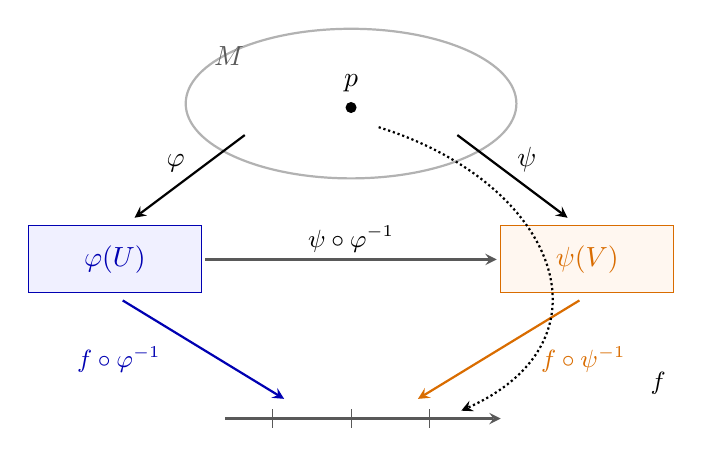
\begin{tikzpicture}[>=stealth,scale=1.0]
% 流形 M
\draw[gray!60,thick] (0,3.4) ellipse (2.1 and 0.95);
\node[gray!70!black] at (-1.55,4.0) {\(M\)};
\fill (0,3.35) circle (2pt);
\node[above=2pt] at (0,3.35) {\(p\)};
% 两张卡
\draw[blue!70!black,fill=blue!6] (-4.1,1.0) rectangle (-1.9,1.85);
\node[blue!70!black] at (-3.0,1.42) {\(\varphi(U)\)};
\draw[orange!85!black,fill=orange!6] (1.9,1.0) rectangle (4.1,1.85);
\node[orange!85!black] at (3.0,1.42) {\(\psi(V)\)};
% 实数轴
\draw[gray!70!black,thick,->] (-1.6,-0.6) -- (1.9,-0.6);
\node[gray!70!black] at (2.25,-0.6) {\(\R\)};
\foreach \x in {-1.0,0,1.0} \draw[gray!70!black] (\x,-0.72) -- (\x,-0.48);
% 箭头
\draw[->,thick] (-1.35,3.0) -- (-2.75,1.95) node[midway,above left=-2pt] {\(\varphi\)};
\draw[->,thick] (1.35,3.0) -- (2.75,1.95) node[midway,above right=-2pt] {\(\psi\)};
\draw[->,thick,blue!70!black] (-2.9,0.9) -- (-0.85,-0.35);
\node[blue!70!black,font=\small] at (-2.95,0.15) {\(f\circ\varphi^{-1}\)};
\draw[->,thick,orange!85!black] (2.9,0.9) -- (0.85,-0.35);
\node[orange!85!black,font=\small] at (2.95,0.15) {\(f\circ\psi^{-1}\)};
\draw[->,thick,gray!70!black] (-1.85,1.42) -- (1.85,1.42);
\node[font=\small] at (0,1.68) {\(\psi\circ\varphi^{-1}\)};
\draw[->,thick,densely dotted] (0.35,3.1) .. controls (2.6,2.4) and (3.4,0.4) .. (1.4,-0.5);
\node[font=\small] at (3.9,-0.15) {\(f\)};
\end{tikzpicture}
\end{center}

\emph{函数从来不直接求导，它先降到某一页地图上；两页地图给出的答案由转移映射对齐。}

\subsection{光滑性只能借卡定义，好在结论与卡无关}

流形上没有现成的微积分，所以``\(f:M\to\R\) 光滑''这句话必须绕道。定义是：对每张卡 \((U,\varphi)\)，复合 \(f\circ\varphi^{-1}\) 作为 \(\R^{d}\) 开集上的普通函数光滑。流形间的映射 \(F:M\to N\) 光滑的意思同样是复合 \(\psi\circ F\circ\varphi^{-1}\) 光滑。

这个定义看着可疑——换张卡会不会结论就变了？不会，而且理由只有一行：两页之间差一个转移映射，\(f\circ\psi^{-1}=(f\circ\varphi^{-1})\circ(\varphi\circ\psi^{-1})\)，光滑函数复合光滑函数仍光滑，反过来同理。条件对账：用到的全部是转移映射光滑且可逆，这两条写在流形的定义里。所以只要在某一张卡上验过，就不必再验第二张。

这是把光滑性押在转移映射上的回报。所有微分学词汇——光滑、微分、临界点、浸入、淹没——都可以搬到任意一页地图上检查，不需要发明一套``弯曲空间专用的微积分''。上面那张图画的就是这件事：两条通往 \(\R\) 的路线，中间由转移映射对齐。

\subsection{函数的微分是切空间上的线性泛函，梯度住在切空间里}

有了光滑性，求导就有了对象。设 \(v\in T_{p}M\) 由曲线 \(\gamma\) 代表，定义

\[
df_{p}(v)=\left.\frac{d}{dt}f\bigl(\gamma(t)\bigr)\right|_{t=0}.
\]

右边只用到一元函数求导，不需要任何额外结构。它与代表元的选取无关：在一张卡下 \(f\circ\gamma=(f\circ\varphi^{-1})\circ(\varphi\circ\gamma)\)，链式法则把结果写成 \(D(f\circ\varphi^{-1})\cdot(\varphi\circ\gamma)'(0)\)，只依赖 \(\gamma\) 的一阶等价类。于是 \(df_{p}\) 是 \(T_{p}M\) 上的线性泛函，在卡下就是熟悉的方向导数。

回到开头的气温。\(df_{p}\) 只是个泛函，要把它变成一个``方向''，得有内积。若 \(M\) 带黎曼度量 \(g\)，Riesz 表示给出唯一的 \(\nabla f(p)\in T_{p}M\) 使得

\[
df_{p}(v)=g_{p}\bigl(\nabla f(p),v\bigr)\quad\text{对一切 } v\in T_{p}M.
\]

这个梯度是切空间里的向量，贴着地表，是你真能迈步的方向。环境空间里那个指向天上的梯度并非算错，它回答的是另一个问题——气温场若延拓到整个 \(\R^{3}\)，在三维中上升最快的方向；把它投影到 \(T_{p}M\) 上，得到的正是流形梯度。顺带说一句，\(\nabla f\) 依赖 \(g\)，而 \(df_{p}\) 不依赖：换一把尺，梯度方向会变，微分本身不变。

\subsection{映射的微分是切空间之间的线性映射，链式法则原样成立}

对流形间的光滑映射 \(F:M\to N\)，同样的手法给出

\[
dF_{p}:T_{p}M\to T_{F(p)}N,\qquad
dF_{p}[\gamma]=[F\circ\gamma].
\]

一个切向量由曲线代表，推过去，取像曲线的速度类。良定义性的检查与上面一样，靠链式法则加转移映射可逆。在卡下写出来，\(dF_{p}\) 就是 \(\psi\circ F\circ\varphi^{-1}\) 的 Jacobi 矩阵——所谓``Jacobi 是一阶最佳线性逼近''，弯曲空间上的版本就是它。

链式法则的形式毫无变化：

\begin{proposition}
设 \(F:M\to N\)、\(G:N\to P\) 光滑，则 \(d(G\circ F)_{p}=dG_{F(p)}\circ dF_{p}\)。
\end{proposition}

证明骨架三步：取代表曲线 \(\gamma\)，两边同时作用在 \([\gamma]\) 上，左边是 \([(G\circ F)\circ\gamma]\)，右边是 \([G\circ(F\circ\gamma)]\)，函数复合的结合律使二者逐字相同。条件对账：全程只用到微分的定义与复合的结合律，没有用到度量、坐标或嵌入。这就是为什么反向传播的推导在流形上不需要修正项——它本来就是链式法则，而链式法则不关心空间弯不弯。

\subsection{子流形的三个来源，各自配一套切空间算法}

本书用到的子流形几乎全部出自三种构造，每种都自带一个算切空间的现成办法。

等值面来自约束。本单元第一节的正则值定理说，若 \(F:\R^{n}\to\R^{k}\) 在 \(F^{-1}(c)\) 上处处满秩，则解集是 \(n-k\) 维子流形；它在 \(p\) 处的切空间恰是 \(\ker dF_{p}\)，也就是与所有约束梯度都正交的那些方向。球面、椭球面、Lyapunov 函数的等高面都属于这一类，约束优化里``可行方向''说的正是这个核。

参数化的像来自生成。若 \(F:\mathcal{A}\to\R^{n}\) 光滑、\(dF\) 处处单射，且 \(F\) 是到像上的同胚，则 \(F(\mathcal{A})\) 是子流形，切空间是 \(dF_{a}\) 的列空间。瑞士卷、以及数据流形的理想化模型都在此列。三个条件里最容易破的是同胚那一条：\(F\) 自交或 \(dF\) 掉秩的地方，像会长出粘连或尖点，流形假设在那里失效。

函数的图来自最朴素的写法。任何 \(h:\R^{d}\to\R^{n-d}\) 的图 \(\set{(x,h(x))}\) 都是子流形，切空间是 \(\set{(v,dh_{x}v)}\)。反过来更值得记住：任何子流形在局部都能写成某个图。这给``局部像欧氏空间''一个最具体的形状。

三套算法里的第二套，与 Part 13 那句``生成映射的 Jacobi 列空间张成局部线性块''是同一句话的两种说法。

\subsection{把流形假设拆成定义、定理和假设三堆}

现在可以给``数据躺在低维流形附近''一个不含糊的分解。设观测由潜变量经光滑映射生成，\(X=F(A)+\varepsilon\)。

若 \(F\) 是嵌入，无噪声样本严格落在子流形 \(F(\mathcal{A})\) 上——这是构造与定义，不需要证明。每个样本附近存在 \(d\) 维切空间作为一阶近似，切空间等于 \(dF_{a}\) 的列空间——这是定理，只要前一条成立就自动成立。而``噪声足够小、\(F\) 确实是嵌入、采样覆盖足够密''，这三条是假设，需要逐条验证，而且可以单独失败：噪声大到与流形厚度同量级，切空间估计就没意义；\(F\) 不单射，近邻关系会把远处的点误判为邻居；采样稀疏，邻接图会断成几块。

具体方法各取所需，也各自继承对应的脆弱点。Isomap 用邻接图上的最短路估计黎曼距离，怕的是短路边。局部线性嵌入拟合局部重构权重，实际上在估计切空间，怕的是噪声压过局部曲率尺度。t-SNE 只保留近邻概率，主动放弃全局几何，于是不怕短路，但也不该拿它的图去读全局形状。选方法，某种意义上就是选你愿意承担哪一类失效。

\subsection{本单元到此为止，弯曲本身还没被量化}

三节铺完了地基：流形给出``局部可拉平''，切空间给出方向，黎曼度量给出长度，而这一节让函数与映射在这套结构上可微，链式法则原封不动。凭这些已经能把``数据有低维结构''``局部可以线性化''``远距离要沿表面走''从口号变成可检验的句子。

还剩一件事没做：弯曲本身有多弯，仍然只有定性的说法。要把它变成一个数，需要曲率——\hyperref[ch:107]{``曲线与曲面几何：弯曲怎样从内蕴被感知''}从最简单的曲线开始，一步步问到``住在曲面上的人能不能测出自己所在的曲面是弯的''。
